\subsection{Factored form}

We will now evaluate the evaluation precision of the following factored rewriting:
\[
	T(x) = 1 + 8x^2\,(x-1)\,(x+1)\,(4x^2 + 2x - 1)^2\, (4x^2 - 2x - 1)^2\,(16x^4 - 20x^2 + 5)^2
\]

\begin{eqnarray*}
T(x) &=& 8.0*x^2*(x - 1.0)*(x + 1.0) \\
 & & * (4.0*x^2 + 2.0*x - 1.0)*(4.0*x^2 + 2.0*x - 1.0) \\
 & & * (4.0*x^2 - 2.0*x - 1.0)*(4.0*x^2 - 2.0*x - 1.0)* \\
 & & * (16.0*x^4 - 20.0*x^2 + 5.0)*(16.0*x^4 - 20.0*x^2 + 5.0) + 1 \\
\end{eqnarray*}

\begin{question}
  \begin{enumerate}[(a)]
  \item Open the file {\tt tchebychev.c} and have a look to the function {\tt REAL factored (REAL x)}
\item Execute the command {\tt ./run.sh FACTORED DOUBLE 24} \newline
The output of this command is given in figure~\ref{fig:factored:double:24}.
\item Compare these results to those obtained with EXPANDED and HORNER versions.
  \end{enumerate}
\end{question}

\begin{figure}[h]
\center 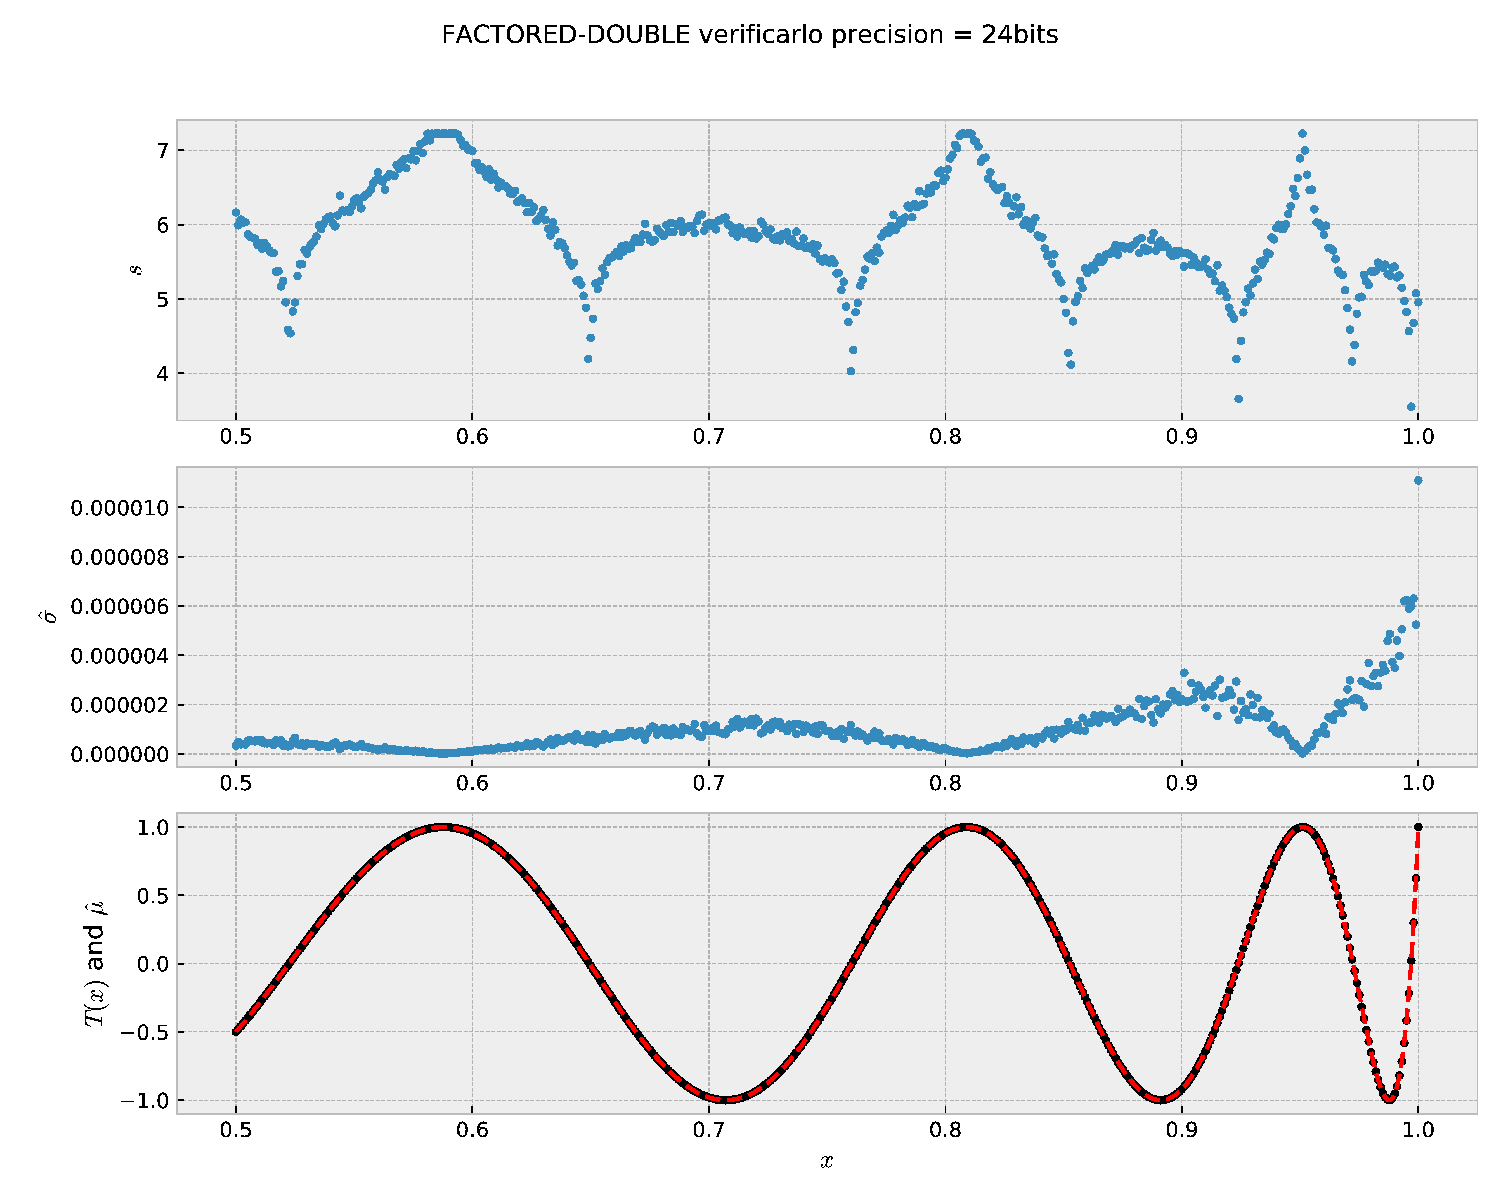
\includegraphics[width=.8\textwidth]{FACTORED-DOUBLE-24.pdf}
  \caption{Evaluation of T(x) in its factored form, compiled in double precision, with a virtual precision of 24}
  \label{fig:factored:double:24}
\end{figure}

\begin{question}
  Explain what happens when $T(x)=1$ for $x\simeq 0.6$,
  $x\simeq 0.8$ et $x\simeq 0.95$.\\~\\
  $\rightarrow$ It is an example where the error is absorbed and the precision and accuracy  of the results are improved.
\end{question}


\begin{question}
  \begin{enumerate}[(a)]
    \item Modify the {\tt run.sh} script to evaluate the  polynomial between $0.99$ and $1$ by $0.00001$ step.
  \item Run the scripts to execute and visualize the results for
    FACTORED, EXPANDED and HORNER with a virtual precision of 53. The results are respectively presented in figure~\ref{fig:factored:double:53:zoom},\ref{fig:expanded:double:53:zoom}
    and~\ref{fig:horner:double:53:zoom}.

\item Reproduce the result with a virtual precision of 24. The results are respectively presented in figure~\ref{fig:factored:double:24:zoom},\ref{fig:expanded:double:24:zoom}
    and~\ref{fig:horner:double:24:zoom}

\end{enumerate}
\end{question}

\begin{figure}[h]
  \center 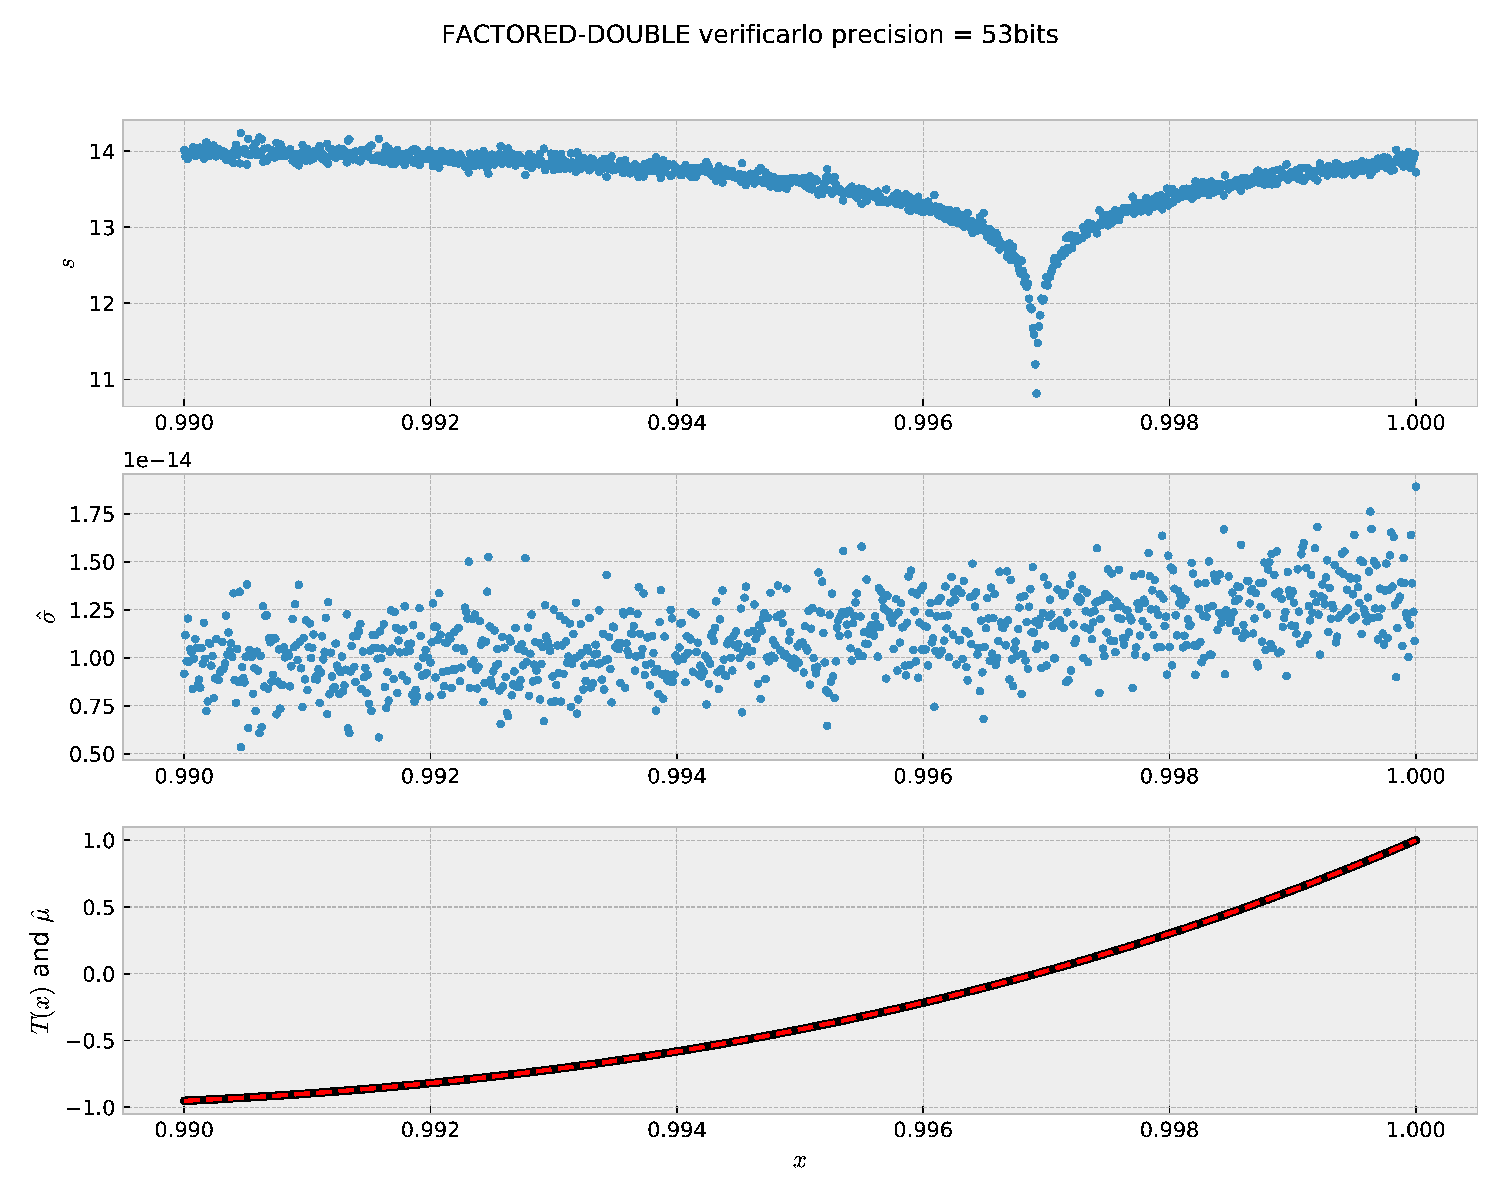
\includegraphics[width=.8\textwidth]{FACTORED-DOUBLE-53-zoom.pdf}
  \caption{Evaluation of T(x) in its factored form, compiled in double
    precision, with a virtual precision of 53}
  \label{fig:factored:double:53:zoom}
\end{figure}

\begin{figure}[h]
  \center 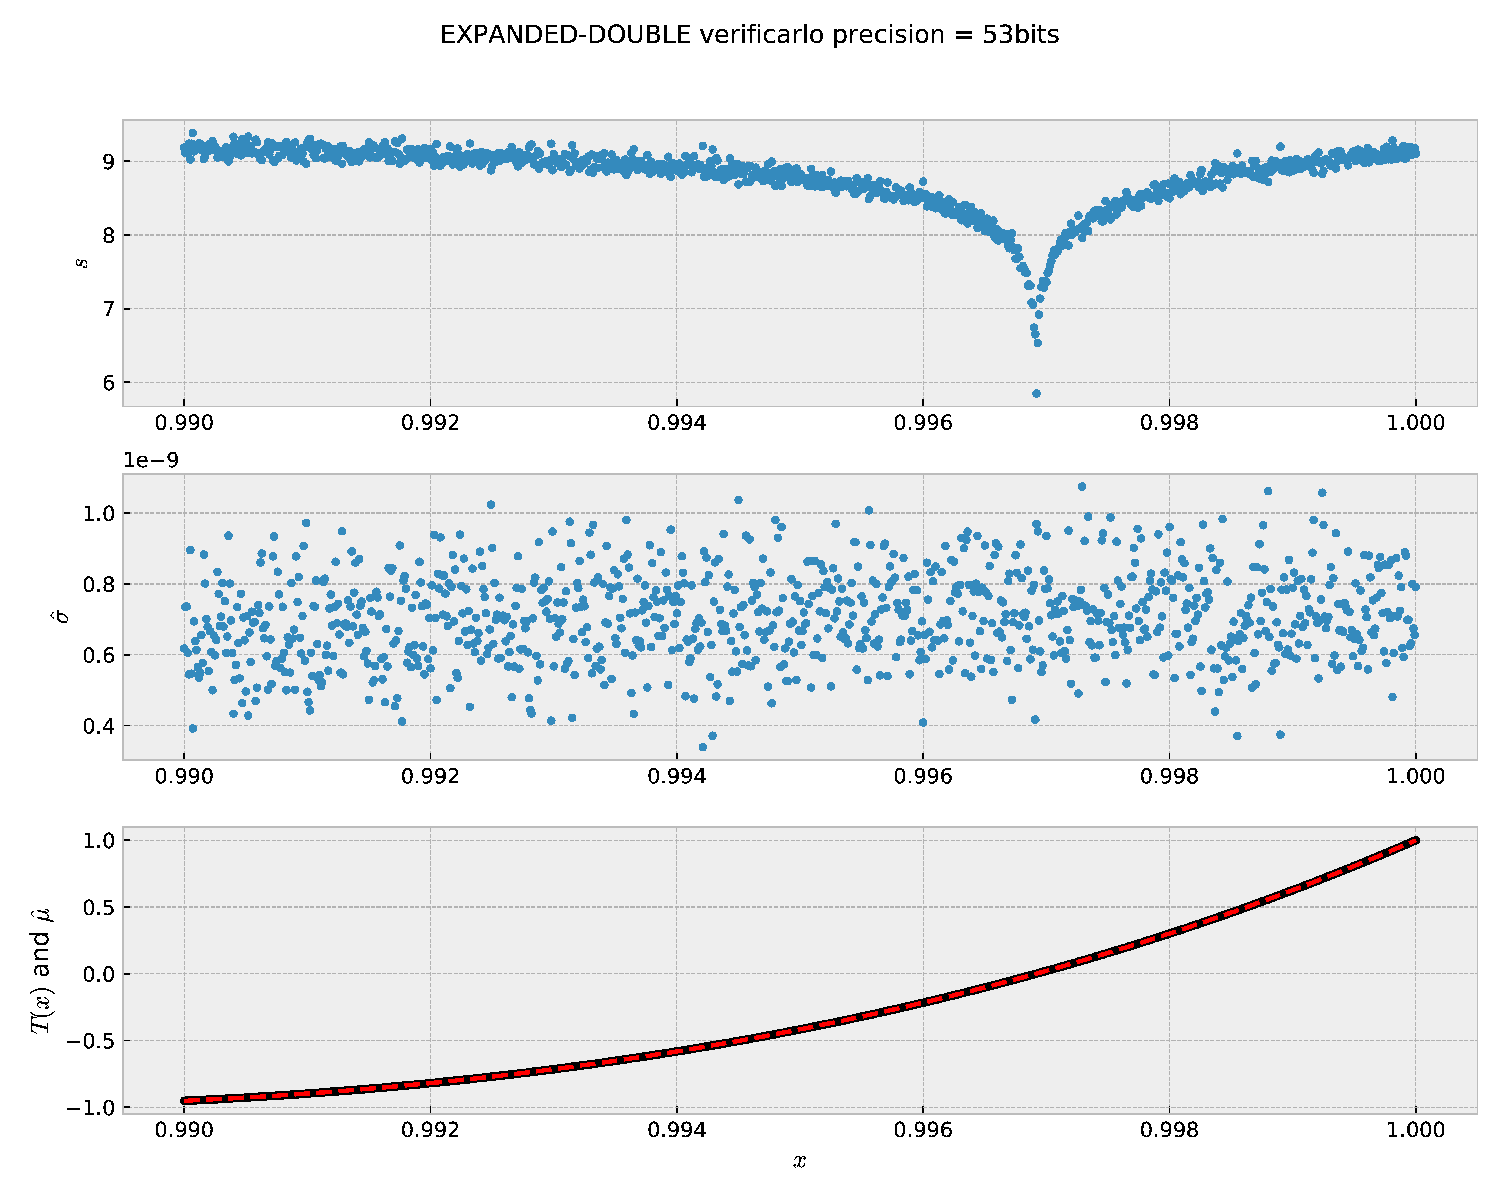
\includegraphics[width=.8\textwidth]{EXPANDED-DOUBLE-53-zoom.pdf}
  \caption{Evaluation of T(x) in its expanded form, compiled in double
    precision, with a virtual precision of 53}
  \label{fig:expanded:double:53:zoom}
\end{figure}

\begin{figure}[h]
  \center 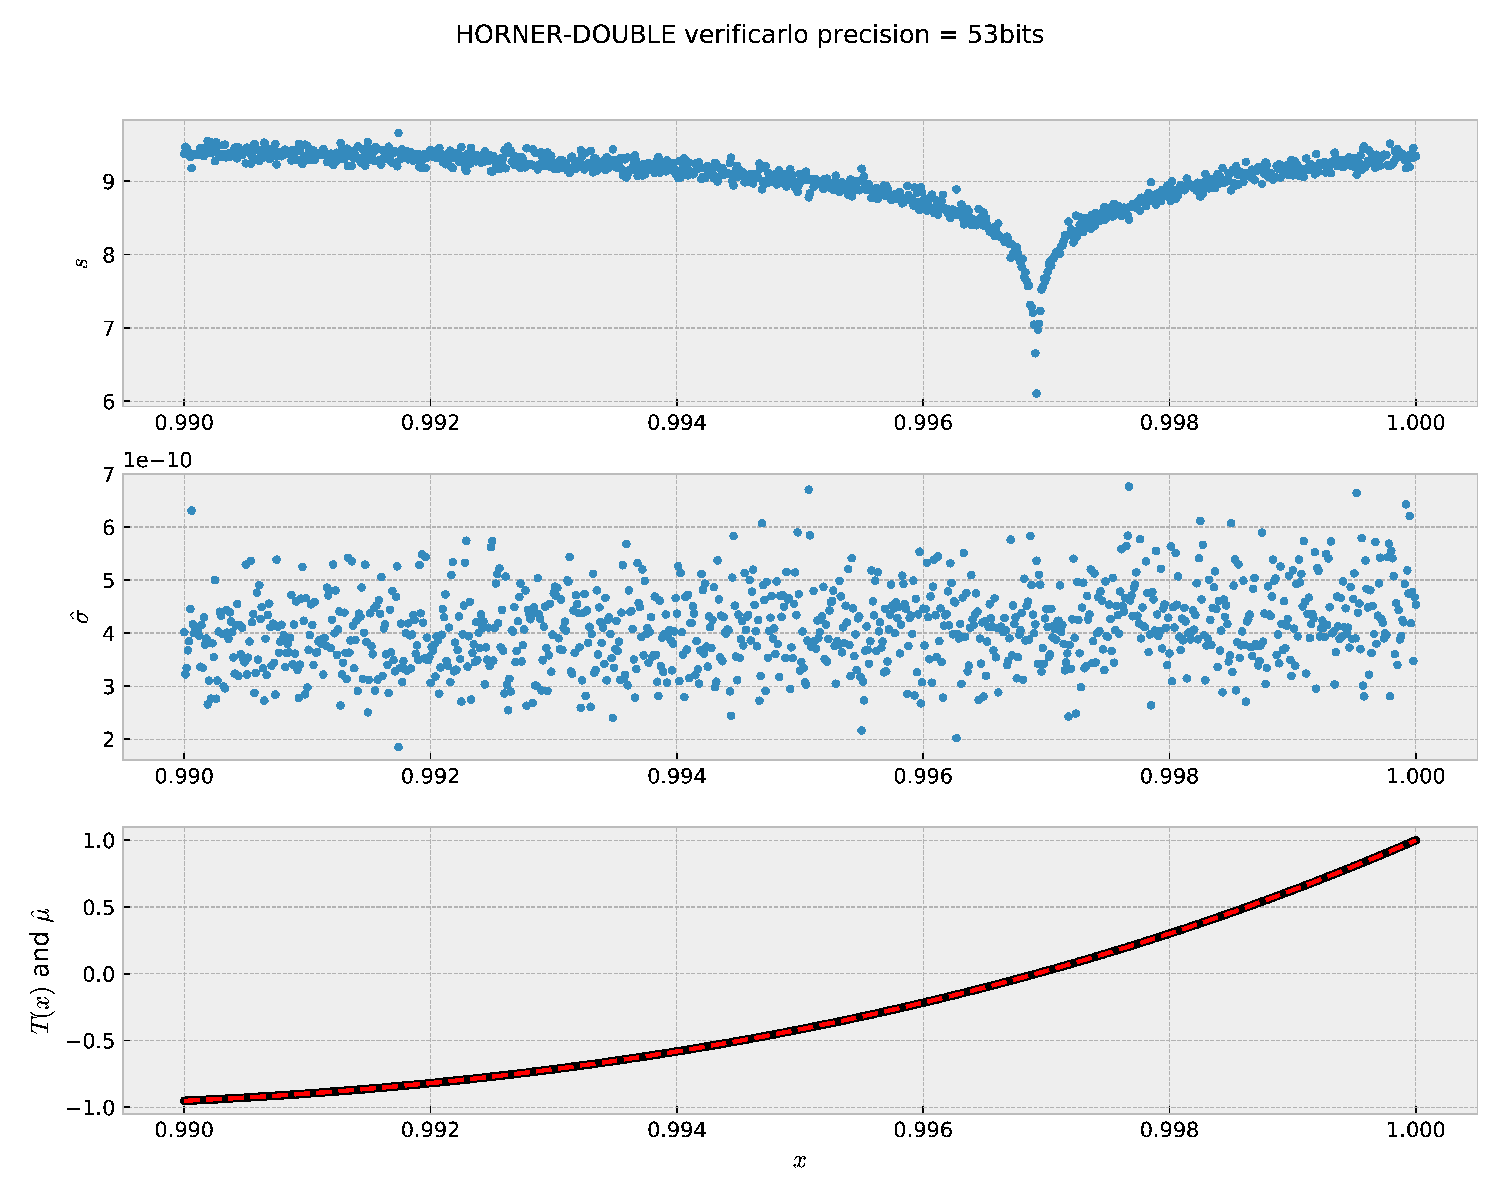
\includegraphics[width=.8\textwidth]{HORNER-DOUBLE-53-zoom.pdf}
  \caption{Evaluation of T(x) using Horner scheme, compiled in double precision,
    with a virtual precision of 53}
  \label{fig:horner:double:53:zoom}
\end{figure}

\begin{figure}[h]
  \center 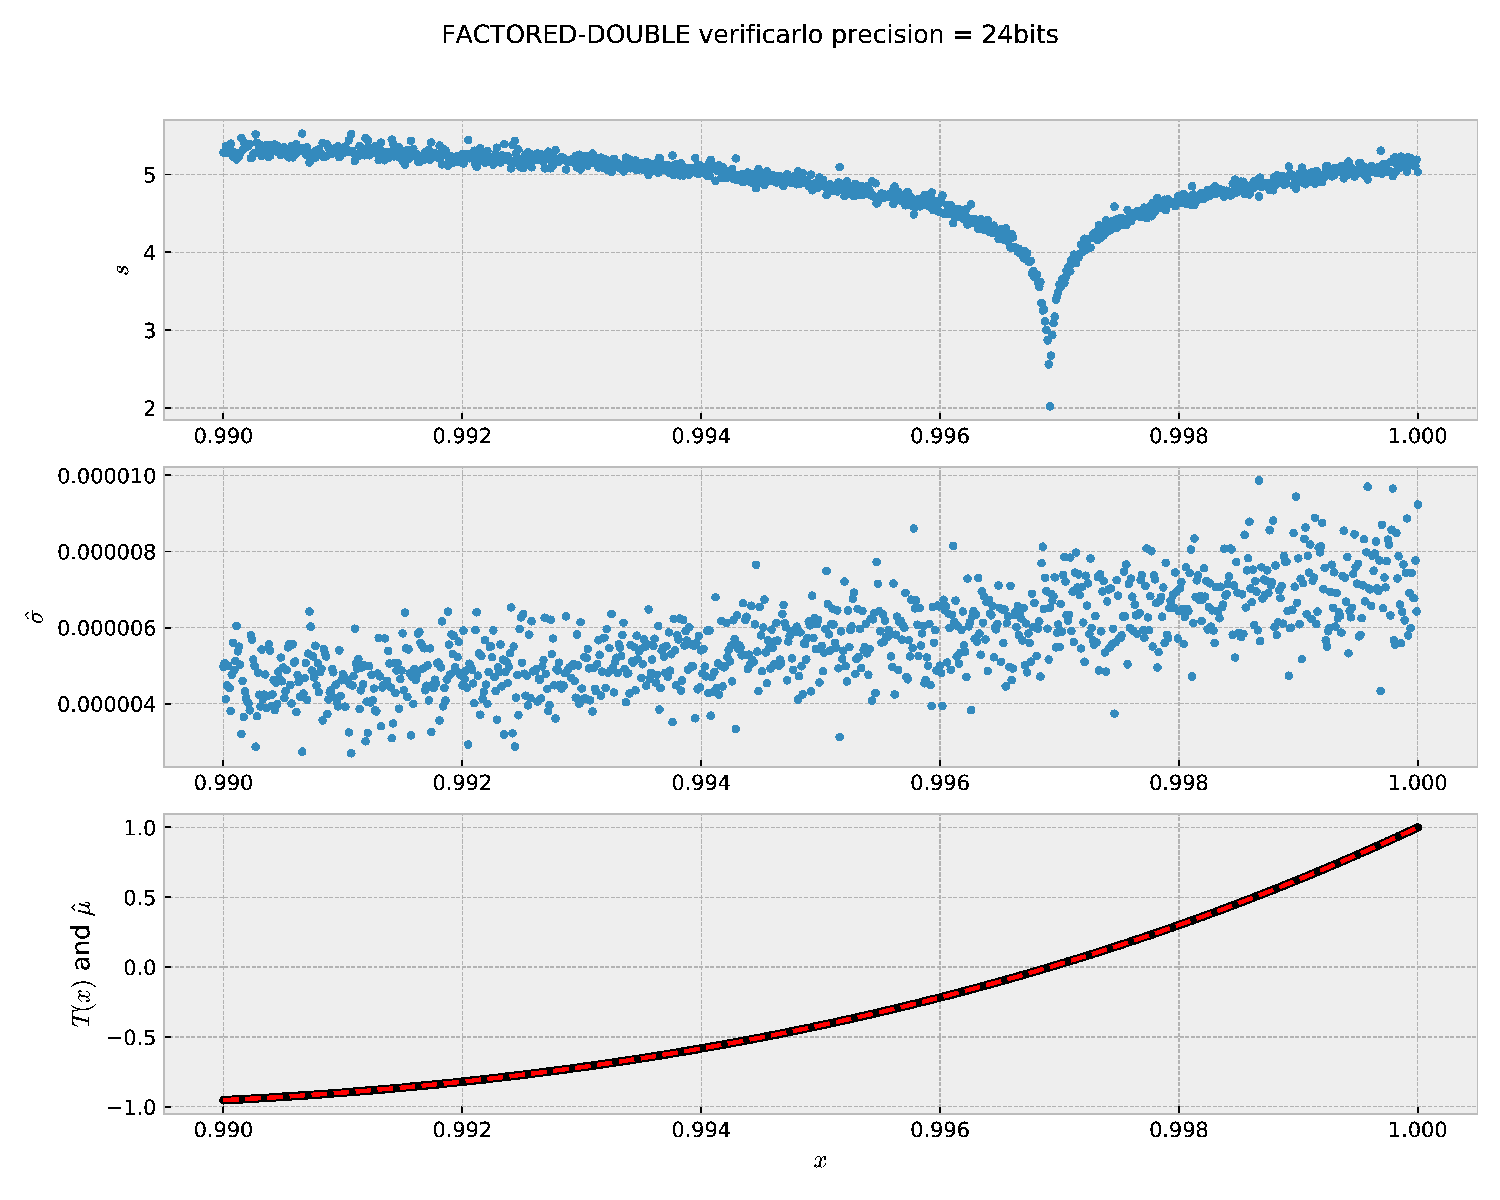
\includegraphics[width=.8\textwidth]{FACTORED-DOUBLE-24-zoom.pdf}
  \caption{Evaluation of T(x) in its factored form, compiled in double
    precision, with a virtual precision of 24}
  \label{fig:factored:double:24:zoom}
\end{figure}

\begin{figure}[h]
  \center 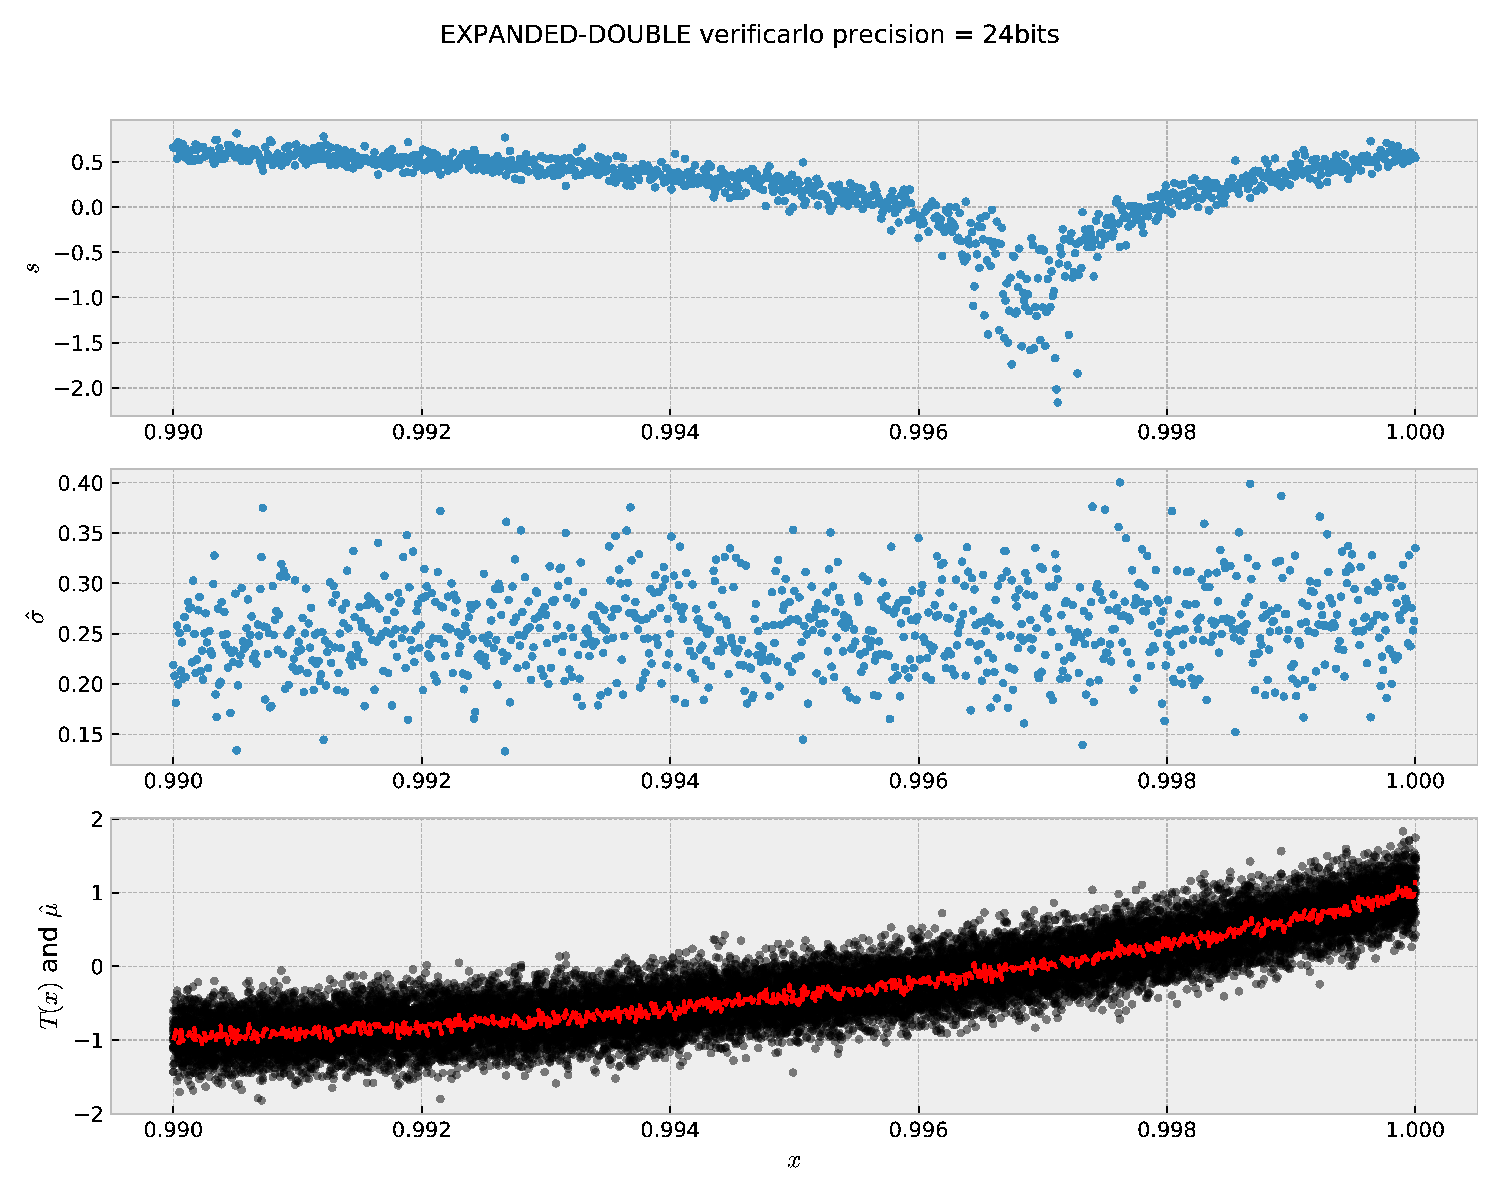
\includegraphics[width=.8\textwidth]{EXPANDED-DOUBLE-24-zoom.pdf}
  \caption{Evaluation of T(x) in its expanded form, compiled in double
    precision, with a virtual precision of 24}
  \label{fig:expanded:double:24:zoom}
\end{figure}

\begin{figure}[h]
  \center 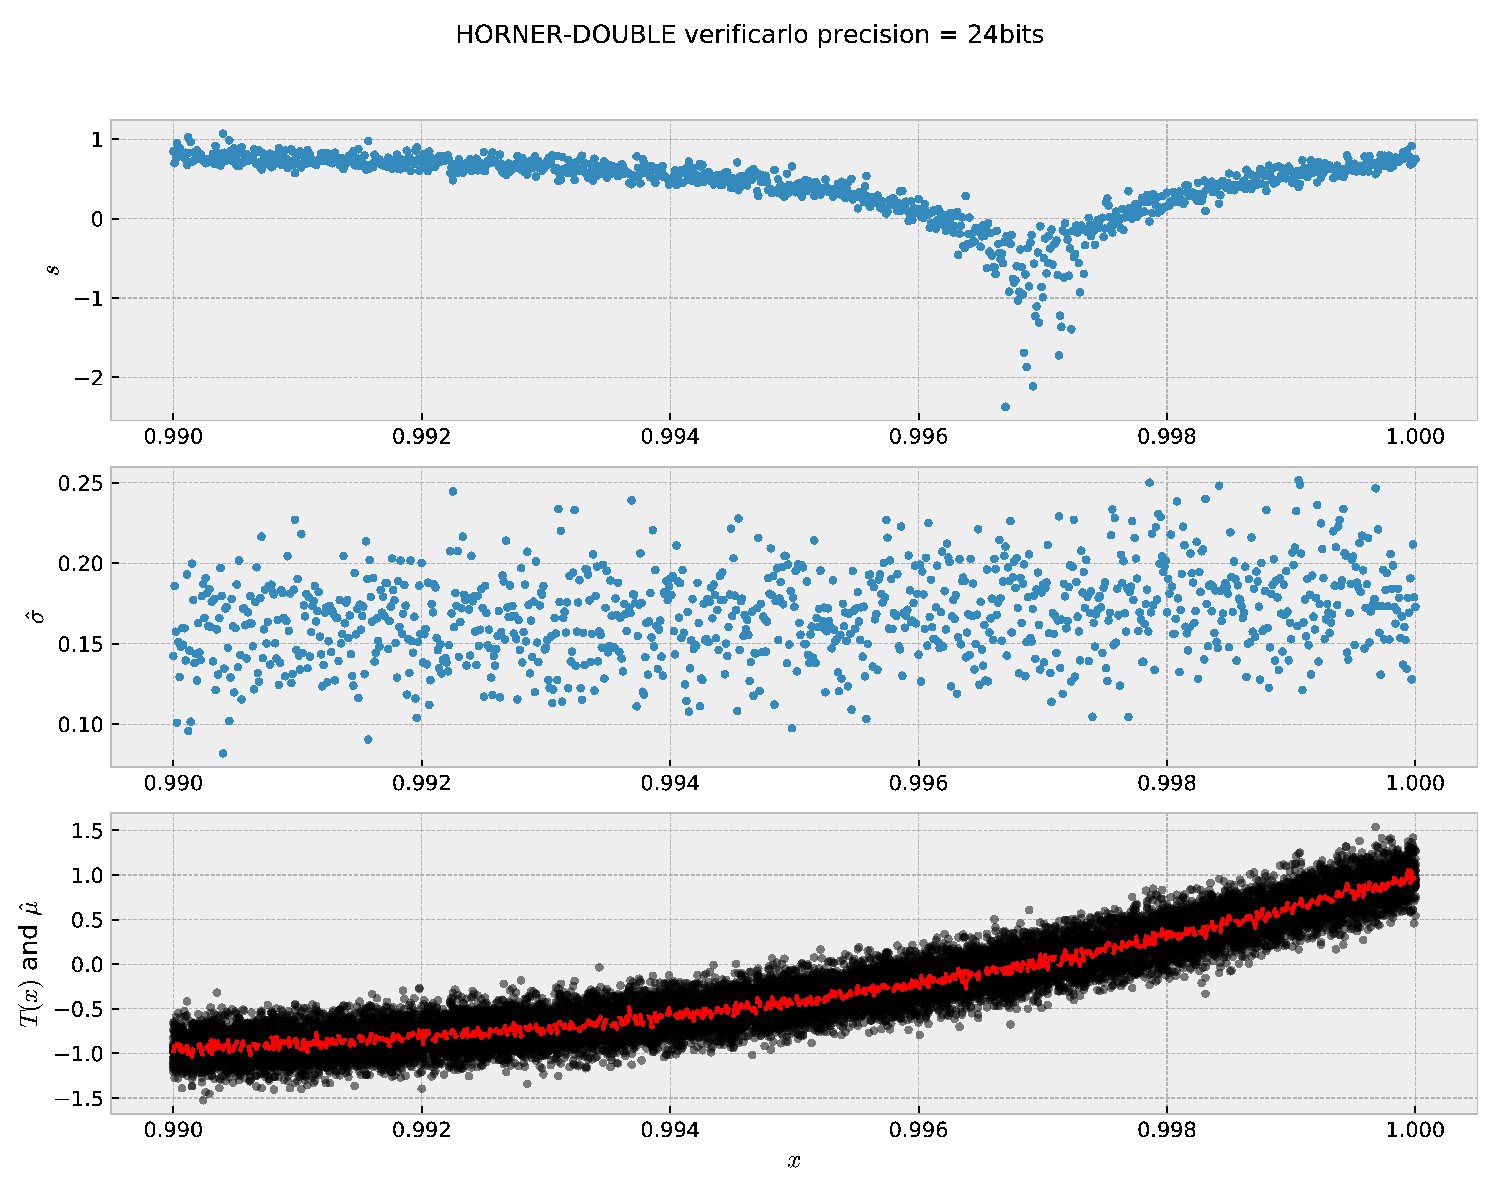
\includegraphics[width=.8\textwidth]{HORNER-DOUBLE-24-zoom.pdf}
  \caption{Evaluation of T(x) using Horner scheme, compiled in double precision,
    with a virtual precision of 24}
    \label{fig:horner:double:24:zoom}
\end{figure}
